%----------------------------------------------------------------
%
%  File    :  chapter6.tex
%
%  Authors : Michael Fuska, FH Campus Wien, Austria% 
%  Created : 13 Feb 2016
%
%  Changed :  
% 
%----------------------------------------------------------------


\chapter{Analyse und Ergebnisse}
\label{ch:Ergebnisse}

%------------------------------------------------------------------------------
%------------------------------ Analysen zur Frage 1

\section{Analysen zur Frage \ref{frage:1}}
\label{sec:Frage1}
\textit{\glqq Eine Aussage über die Sicherheit und die Vertrauenswürdigkeit der iOS Devices(iPhone, iPad) tätigen zu können. Und in wieweit die veröffentlichten JBs einen Einfluss darauf hatten. \grqq{}}

G1.1: \textit{\glqq Wie weit hängt die Sicherheit und die Vertrauenswürdigkeit des iOS Device von der Hardware des Device ab?\grqq{}}

\begin{table}[htp!]
    \begin{center}
        \begin{tabular}{|p{30mm}|p{27mm}|p{12mm}|p{18mm}|p{2cm}|p{22mm}|} \hline
            \textbf{iOS Device} & \textbf{Verkaufsstart} & \textbf{initial iOS} & \textbf{Secure Enclave} & \textbf{Prozessor}  & \textbf{\#Tage JB} \\ \hline
            \textbf{iPhone} & 29.06.2007  & 1.0 & nA & Samsung SSL8900 & 11\\ \hline
            \textbf{iPhone 3G} & 11.07.2008 & 2.0 & nA & Samsung SSL8900 & 9\\ \hline
            \textbf{iPhone 3GS} & 19.06.2009 & 3.0 & nA & Samsung SSL8920 & 14\\ \hline
            \textbf{iPhone 4} & 01.08.2010 & 4.0 & nA & Apple A4 & 38 \\ \hline
            \textbf{iPhone 4s} & 20.01.2012 & 5.0 & nA & Apple A5 & 98 \\ \hline 
            \textbf{iPhone 5} & 21.09.2012 & 6.0 & nA & Apple A6 & 136 \\ \hline
            \textbf{iPhone 5c} & 22.12.2013 & 7.0 & nA & Apple A6 & 93 \\ \hline
            \textbf{iPhone 5s} & 22.12.2013 & 7.0 & A & Apple A7 & 93 \\ \hline
            \textbf{iPhone 6} & 19.09.2014 & 8.0 & A & Apple A8 & 33\\ \hline
            \textbf{iPhone 6 Plus} & 19.09.2014 & 8.0 & A & Apple A8 & 33\\ \hline
            \textbf{iPhone 6s} & 25.09.2016 & 9.0 & A & Apple A9 & 19\\ \hline
            \textbf{iPhone 6s Plus} & 25.09.2016 & 9.0 & A & Apple A9 & 19\\ \hline
            \textbf{iPhone SE} & 31.03.2016 & 9.0 & A & Apple A9 & nA\\ \hline  
        \end{tabular} 
        \caption{Auflistung iOS Device/ Verkaufsstart/ initiale iOS/ Prozessor/ \#Tage bis zum JB}
        \label{tab:iOSHW}
    \end{center}
\end{table}
In der Tabelle \ref{tab:iOSHW} werden alle iOS Devices angeführt und in Abhängigkeit von den Verkaufszeitpunkt, iOS Auslieferungsversion und der Prozessors des iDevice aufgelistet. Weiters wird auch angeführt, ob dieses Device einen Koprozessor mit Secure Enclave implementiert hat und wie lange die JB Community benötigte, um ein JB auf diesem Device zu installieren.\par
Die Tabelle \ref{tab:iOSHW} alleine gibt noch keinen Aufschluss über den Zusammenhang zwischen der Sicherheit des Systems und der verwendeten iOS Hardware. Aber im Zusammenhang mit der installierten iOS Version können Rückschlüsse über die Sicherheit und Vertrauenswürdigkeit des Systems getroffen werden.

\begin{figure}[htbp]
        \centering
                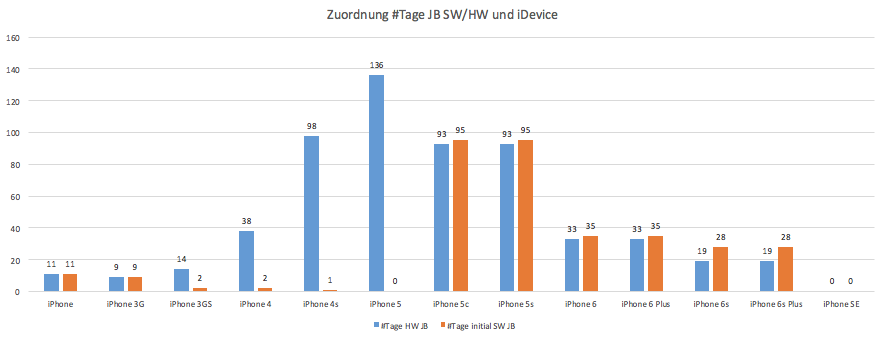
\includegraphics[scale=0.4]{Bilder/iDeviceJB-SW-HW.png}
         \caption{Auflistung iOS Device/ Initiale iOS/ \#Tage bis zum HW JB / \#Tage bis zum SW JB}
        \label{tab:AuflistungDeviceHWiOS}      
\end{figure}


%\begin{table}[htp!]
%    \begin{center}
%        \begin{tabular}{|p{30mm}|p{12mm}|p{18mm}|p{18mm}|} \hline
%            \textbf{iOS Device} & \textbf{initial iOS} & \textbf{\#Tage JB HW} & \textbf{\#Tage JB SW} \\ \hline
%            \textbf{iPhone} & 1.0 & 11 & 11\\ \hline
%            \textbf{iPhone 3G} & 2.0 & 9 & 9\\ \hline
%            \textbf{iPhone 3GS} & 3.0 & 14 & 2\\ \hline
%            \textbf{iPhone 4} & 4.0 & 38 & 2\\ \hline
%            \textbf{iPhone 4s} & 5.0 & 98 & 1\\ \hline 
%            \textbf{iPhone 5} & 6.0 & 136 & 0\\ \hline
%            \textbf{iPhone 5c} & 7.0 & 93 & 95\\ \hline
%            \textbf{iPhone 5s} & 7.0 & 93 & 95\\ \hline
%            \textbf{iPhone 6} & 8.0 & 33 & 35\\ \hline
%            \textbf{iPhone 6 Plus} & 8.0 & 33 & 35\\ \hline
%            \textbf{iPhone 6s} & 9.0 & 19 & 28\\ \hline
%            \textbf{iPhone 6s Plus} & 9.0 & 19 & 28\\ \hline
%            \textbf{iPhone SE} & 9.0 & nA & nA \\ \hline  
%        \end{tabular} 
%        \caption{Auflistung iOS Device/ Initiale iOS/ \#Tage bis zum HW JB / \#Tage bis zum SW JB}
%        \label{tab:AuflistungDeviceHWiOS}
%    \end{center}
%\end{table}

G1.2: \textit{\glqq Wie weit hängt die Sicherheit und die Vertrauenswürdigkeit des iOS Device von Apples mobilen Betriebssystem (iOS) ab?\grqq{}}
\begin{table}[htp!]
    \begin{center}
        \begin{tabular}{|l|l|l|} \hline
         \textbf{iOS Version} & \textbf{Veröffentilicht} & \textbf{Tage JB}\\ \hline    
        1.0 & 29.06.2007 & 11\\ \hline 
        2.0 & 11.07.2008	& 9\\ \hline 
        3.0 & 17.06.2009	& 2\\ \hline 
        4.0 & 21.06.2010 & 2\\ \hline 
        5.0 & 12.10.2011	& 1\\ \hline 
        6.0 & 19.09.2012	& 0\\ \hline 
        7.0 & 18.09.2013	& 95\\ \hline 
        7.1-7.1.2 & 29.05.2014 & 25\\ \hline 
        8.0 & 17.09.2014	& 35\\ \hline 
        8.1.1-8.4 & 17.11.2014	& 12\\ \hline 
        9.0 & 16.09.2015	& 28\\ \hline
       %  9.0.1 & 23.09.2015 & nA \\ \hline
       %  9.0.2 & 30.09.2015 & nA \\ \hline 
        9.1 & 21.10.2015	& 142\\ \hline 
       %  9.2 & 08.12,2015 & nA\\ \hline
       % 9.2.1 & 18.02.2016 & nA \\ \hline
       %  9.3 & 21.03,016 & nA\\ \hline 
       % 9.3.1 & 31.03.2016 & nA\\ \hline
       % 9.3.2 & 17.05.2016 & nA \\ \hline
        \end{tabular} 
        \caption{Sicherheitszusammenhang iOS Version und JB}
        \label{tab:iOSVersion}
    \end{center}
\end{table}

G1.3: \textit{\glqq Wie weit hängt die Sicherheit und die Vertrauenswürdigkeit des iOS Device von den veröffentlichten Jailbreaks(JBs) ab?\grqq{}}

         
\begin{figure}[htbp]
        \centering
                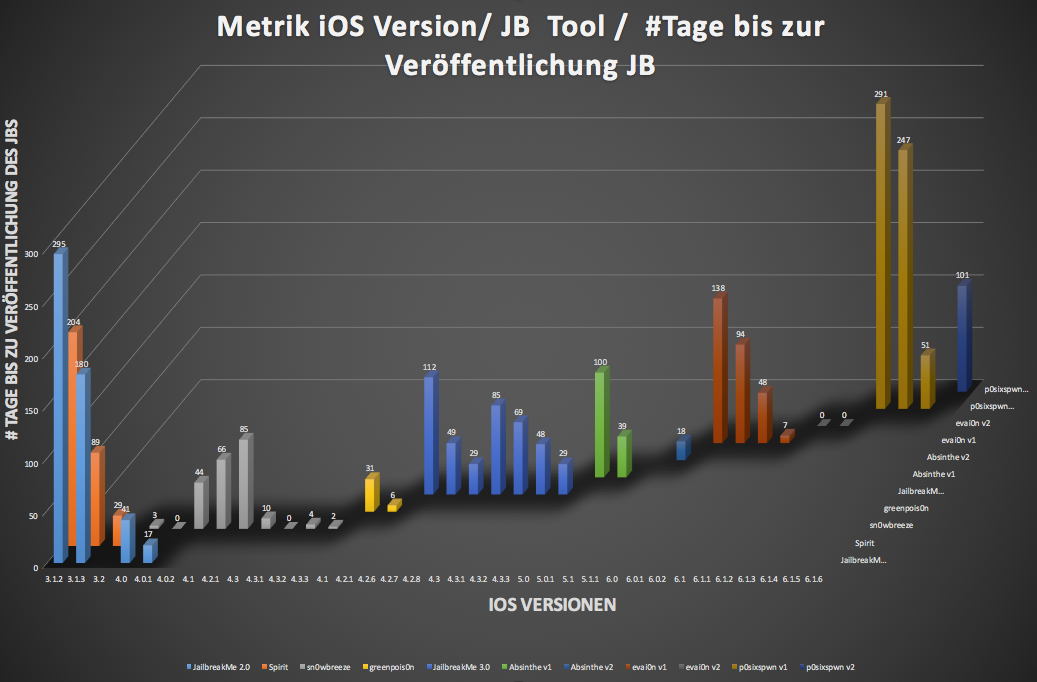
\includegraphics[height=11cm]{Bilder/Frage1_1.png}
        \caption{iOS Version / JB / Tage}
        \label{fig:AnalyseiOSJB1}        
\end{figure}

\begin{figure}[htbp]
        \centering
                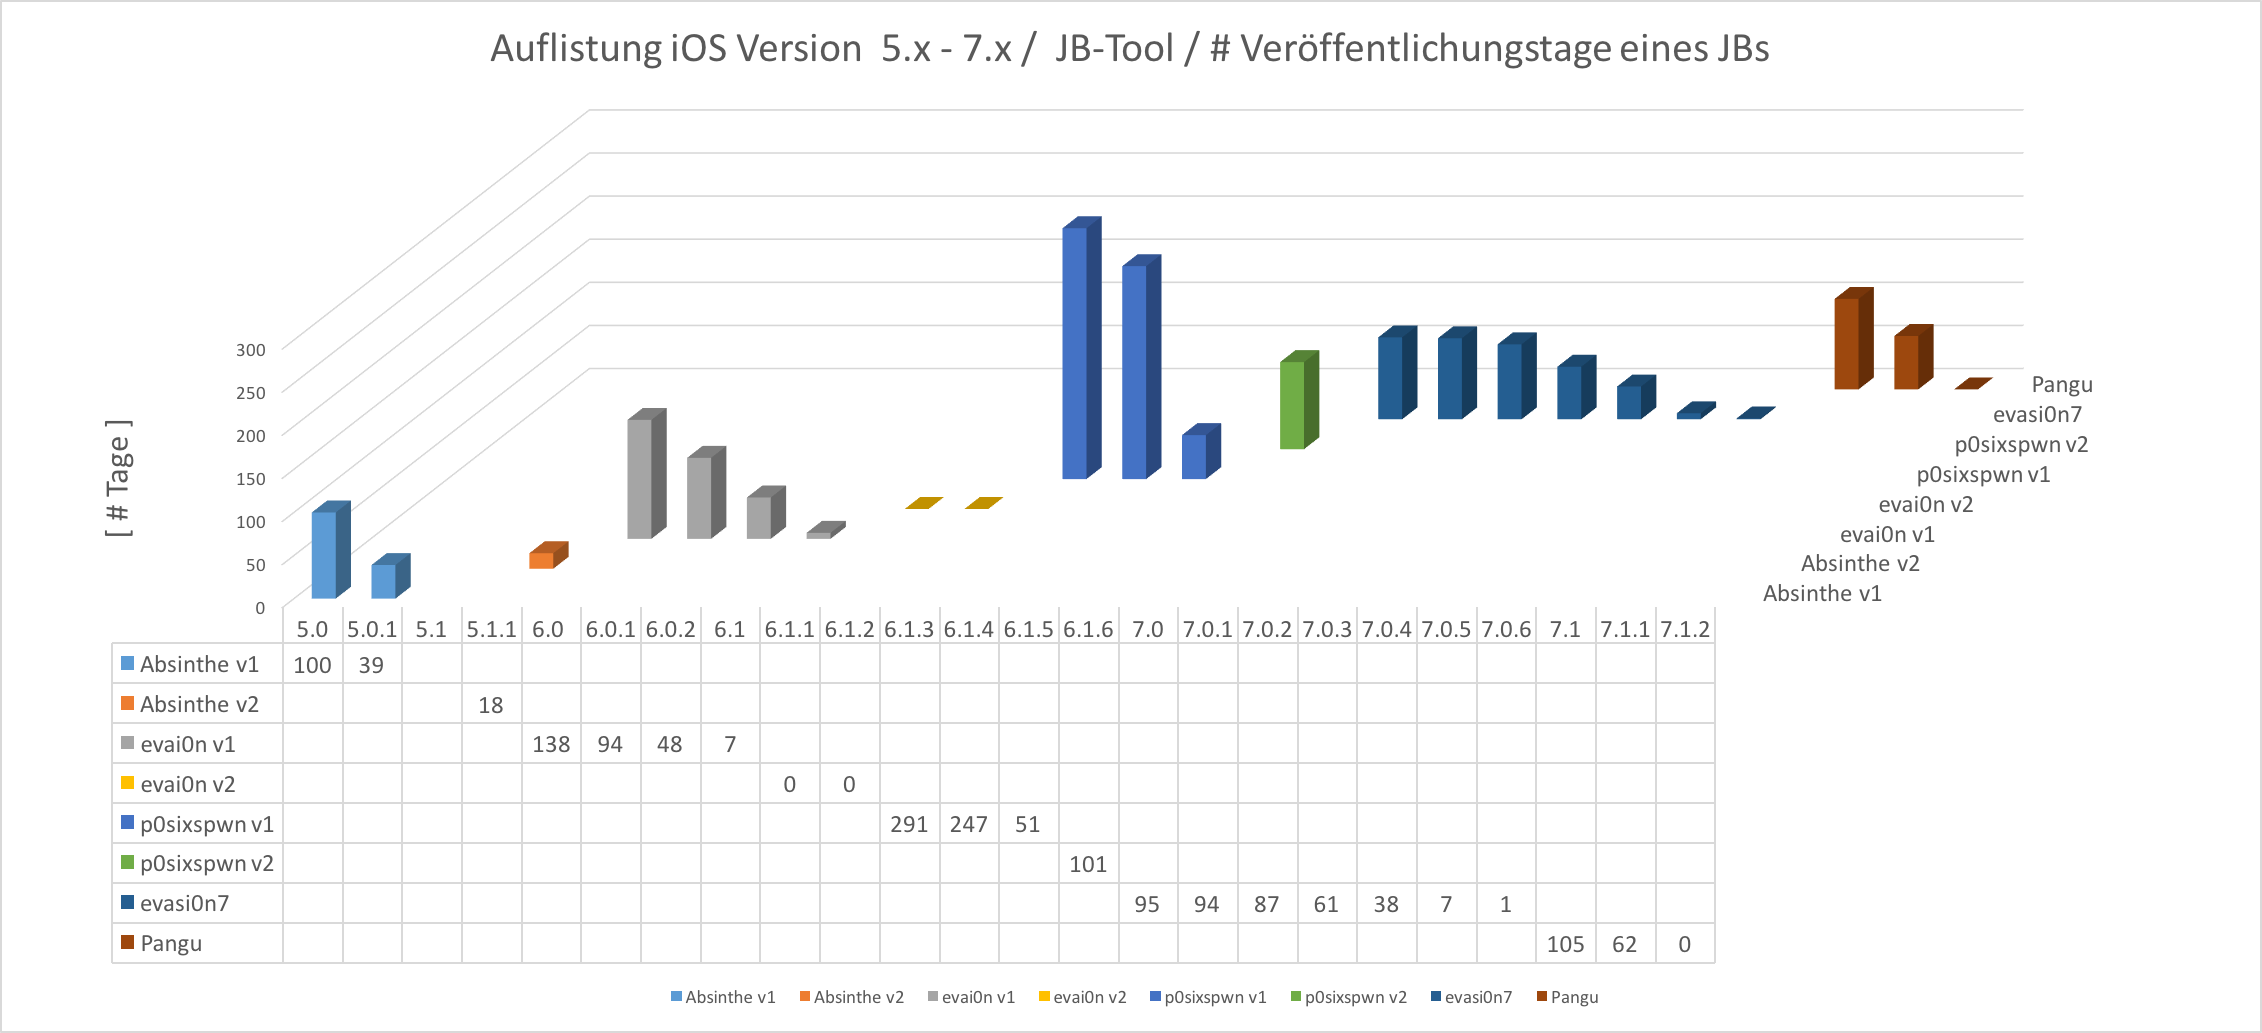
\includegraphics[height=10cm]{Bilder/Frage1_2.png}
        \caption{iOS Version / JB / Tage}
        \label{fig:AnalyseiOSJB2}
\end{figure}

\section{Frage 2}
\label{sec:Frage2}
\textit{\glqq Welche Auswirkung haben die von Apple eingeführten Sicherheitsmechanismen und Sicherheitsupdates auf die Sicherheit des Systems?\grqq{}} 
            
     
\begin{description}
    \item[\parbox{\textwidth} {Antwort kurz INFO Katharina}]~\par
        \begin{itemize}
                \item Zuordnung Bugs / Sicherheitsmechanismen Ausreißer in den Stats Veröffentlichung \#Tage JB  
        \end{itemize}
\end{description} 
        


\section{Frage 3}
\label{sec:Frage3}
\textit{\glqq Welche Auswirkung hat die Veröffentlichung eines JB auf die Sicherheit des Devices?\grqq{}}
\begin{description}
    \item[\parbox{\textwidth} {Antwort kurz INFO Katharina}]~\par
        \begin{itemize}
                \item \#Tage Gültigkeit eines JB -> Erklärung Dauer / Ausreißer
                \item \#Geschlossene Bugs (Apple / JB)   -> Erklärung 
        \end{itemize}
\end{description} 
 